% Options for packages loaded elsewhere
\PassOptionsToPackage{unicode}{hyperref}
\PassOptionsToPackage{hyphens}{url}
\PassOptionsToPackage{dvipsnames,svgnames,x11names}{xcolor}
%
\documentclass[
]{article}

\usepackage{amsmath,amssymb}
\usepackage{iftex}
\ifPDFTeX
  \usepackage[T1]{fontenc}
  \usepackage[utf8]{inputenc}
  \usepackage{textcomp} % provide euro and other symbols
\else % if luatex or xetex
  \usepackage{unicode-math}
  \defaultfontfeatures{Scale=MatchLowercase}
  \defaultfontfeatures[\rmfamily]{Ligatures=TeX,Scale=1}
\fi
\usepackage{lmodern}
\ifPDFTeX\else  
    % xetex/luatex font selection
\fi
% Use upquote if available, for straight quotes in verbatim environments
\IfFileExists{upquote.sty}{\usepackage{upquote}}{}
\IfFileExists{microtype.sty}{% use microtype if available
  \usepackage[]{microtype}
  \UseMicrotypeSet[protrusion]{basicmath} % disable protrusion for tt fonts
}{}
\makeatletter
\@ifundefined{KOMAClassName}{% if non-KOMA class
  \IfFileExists{parskip.sty}{%
    \usepackage{parskip}
  }{% else
    \setlength{\parindent}{0pt}
    \setlength{\parskip}{6pt plus 2pt minus 1pt}}
}{% if KOMA class
  \KOMAoptions{parskip=half}}
\makeatother
\usepackage{xcolor}
\setlength{\emergencystretch}{3em} % prevent overfull lines
\setcounter{secnumdepth}{-\maxdimen} % remove section numbering
% Make \paragraph and \subparagraph free-standing
\ifx\paragraph\undefined\else
  \let\oldparagraph\paragraph
  \renewcommand{\paragraph}[1]{\oldparagraph{#1}\mbox{}}
\fi
\ifx\subparagraph\undefined\else
  \let\oldsubparagraph\subparagraph
  \renewcommand{\subparagraph}[1]{\oldsubparagraph{#1}\mbox{}}
\fi

\usepackage{color}
\usepackage{fancyvrb}
\newcommand{\VerbBar}{|}
\newcommand{\VERB}{\Verb[commandchars=\\\{\}]}
\DefineVerbatimEnvironment{Highlighting}{Verbatim}{commandchars=\\\{\}}
% Add ',fontsize=\small' for more characters per line
\usepackage{framed}
\definecolor{shadecolor}{RGB}{241,243,245}
\newenvironment{Shaded}{\begin{snugshade}}{\end{snugshade}}
\newcommand{\AlertTok}[1]{\textcolor[rgb]{0.68,0.00,0.00}{#1}}
\newcommand{\AnnotationTok}[1]{\textcolor[rgb]{0.37,0.37,0.37}{#1}}
\newcommand{\AttributeTok}[1]{\textcolor[rgb]{0.40,0.45,0.13}{#1}}
\newcommand{\BaseNTok}[1]{\textcolor[rgb]{0.68,0.00,0.00}{#1}}
\newcommand{\BuiltInTok}[1]{\textcolor[rgb]{0.00,0.23,0.31}{#1}}
\newcommand{\CharTok}[1]{\textcolor[rgb]{0.13,0.47,0.30}{#1}}
\newcommand{\CommentTok}[1]{\textcolor[rgb]{0.37,0.37,0.37}{#1}}
\newcommand{\CommentVarTok}[1]{\textcolor[rgb]{0.37,0.37,0.37}{\textit{#1}}}
\newcommand{\ConstantTok}[1]{\textcolor[rgb]{0.56,0.35,0.01}{#1}}
\newcommand{\ControlFlowTok}[1]{\textcolor[rgb]{0.00,0.23,0.31}{#1}}
\newcommand{\DataTypeTok}[1]{\textcolor[rgb]{0.68,0.00,0.00}{#1}}
\newcommand{\DecValTok}[1]{\textcolor[rgb]{0.68,0.00,0.00}{#1}}
\newcommand{\DocumentationTok}[1]{\textcolor[rgb]{0.37,0.37,0.37}{\textit{#1}}}
\newcommand{\ErrorTok}[1]{\textcolor[rgb]{0.68,0.00,0.00}{#1}}
\newcommand{\ExtensionTok}[1]{\textcolor[rgb]{0.00,0.23,0.31}{#1}}
\newcommand{\FloatTok}[1]{\textcolor[rgb]{0.68,0.00,0.00}{#1}}
\newcommand{\FunctionTok}[1]{\textcolor[rgb]{0.28,0.35,0.67}{#1}}
\newcommand{\ImportTok}[1]{\textcolor[rgb]{0.00,0.46,0.62}{#1}}
\newcommand{\InformationTok}[1]{\textcolor[rgb]{0.37,0.37,0.37}{#1}}
\newcommand{\KeywordTok}[1]{\textcolor[rgb]{0.00,0.23,0.31}{#1}}
\newcommand{\NormalTok}[1]{\textcolor[rgb]{0.00,0.23,0.31}{#1}}
\newcommand{\OperatorTok}[1]{\textcolor[rgb]{0.37,0.37,0.37}{#1}}
\newcommand{\OtherTok}[1]{\textcolor[rgb]{0.00,0.23,0.31}{#1}}
\newcommand{\PreprocessorTok}[1]{\textcolor[rgb]{0.68,0.00,0.00}{#1}}
\newcommand{\RegionMarkerTok}[1]{\textcolor[rgb]{0.00,0.23,0.31}{#1}}
\newcommand{\SpecialCharTok}[1]{\textcolor[rgb]{0.37,0.37,0.37}{#1}}
\newcommand{\SpecialStringTok}[1]{\textcolor[rgb]{0.13,0.47,0.30}{#1}}
\newcommand{\StringTok}[1]{\textcolor[rgb]{0.13,0.47,0.30}{#1}}
\newcommand{\VariableTok}[1]{\textcolor[rgb]{0.07,0.07,0.07}{#1}}
\newcommand{\VerbatimStringTok}[1]{\textcolor[rgb]{0.13,0.47,0.30}{#1}}
\newcommand{\WarningTok}[1]{\textcolor[rgb]{0.37,0.37,0.37}{\textit{#1}}}

\providecommand{\tightlist}{%
  \setlength{\itemsep}{0pt}\setlength{\parskip}{0pt}}\usepackage{longtable,booktabs,array}
\usepackage{calc} % for calculating minipage widths
% Correct order of tables after \paragraph or \subparagraph
\usepackage{etoolbox}
\makeatletter
\patchcmd\longtable{\par}{\if@noskipsec\mbox{}\fi\par}{}{}
\makeatother
% Allow footnotes in longtable head/foot
\IfFileExists{footnotehyper.sty}{\usepackage{footnotehyper}}{\usepackage{footnote}}
\makesavenoteenv{longtable}
\usepackage{graphicx}
\makeatletter
\def\maxwidth{\ifdim\Gin@nat@width>\linewidth\linewidth\else\Gin@nat@width\fi}
\def\maxheight{\ifdim\Gin@nat@height>\textheight\textheight\else\Gin@nat@height\fi}
\makeatother
% Scale images if necessary, so that they will not overflow the page
% margins by default, and it is still possible to overwrite the defaults
% using explicit options in \includegraphics[width, height, ...]{}
\setkeys{Gin}{width=\maxwidth,height=\maxheight,keepaspectratio}
% Set default figure placement to htbp
\makeatletter
\def\fps@figure{htbp}
\makeatother

\makeatletter
\makeatother
\makeatletter
\makeatother
\makeatletter
\@ifpackageloaded{caption}{}{\usepackage{caption}}
\AtBeginDocument{%
\ifdefined\contentsname
  \renewcommand*\contentsname{Table of contents}
\else
  \newcommand\contentsname{Table of contents}
\fi
\ifdefined\listfigurename
  \renewcommand*\listfigurename{List of Figures}
\else
  \newcommand\listfigurename{List of Figures}
\fi
\ifdefined\listtablename
  \renewcommand*\listtablename{List of Tables}
\else
  \newcommand\listtablename{List of Tables}
\fi
\ifdefined\figurename
  \renewcommand*\figurename{Figure}
\else
  \newcommand\figurename{Figure}
\fi
\ifdefined\tablename
  \renewcommand*\tablename{Table}
\else
  \newcommand\tablename{Table}
\fi
}
\@ifpackageloaded{float}{}{\usepackage{float}}
\floatstyle{ruled}
\@ifundefined{c@chapter}{\newfloat{codelisting}{h}{lop}}{\newfloat{codelisting}{h}{lop}[chapter]}
\floatname{codelisting}{Listing}
\newcommand*\listoflistings{\listof{codelisting}{List of Listings}}
\makeatother
\makeatletter
\@ifpackageloaded{caption}{}{\usepackage{caption}}
\@ifpackageloaded{subcaption}{}{\usepackage{subcaption}}
\makeatother
\makeatletter
\@ifpackageloaded{tcolorbox}{}{\usepackage[skins,breakable]{tcolorbox}}
\makeatother
\makeatletter
\@ifundefined{shadecolor}{\definecolor{shadecolor}{rgb}{.97, .97, .97}}
\makeatother
\makeatletter
\makeatother
\makeatletter
\makeatother
\ifLuaTeX
  \usepackage{selnolig}  % disable illegal ligatures
\fi
\IfFileExists{bookmark.sty}{\usepackage{bookmark}}{\usepackage{hyperref}}
\IfFileExists{xurl.sty}{\usepackage{xurl}}{} % add URL line breaks if available
\urlstyle{same} % disable monospaced font for URLs
\hypersetup{
  pdftitle={Biostat 212a Homework 2},
  pdfauthor={Wenqiang Ge UID:106371961},
  colorlinks=true,
  linkcolor={blue},
  filecolor={Maroon},
  citecolor={Blue},
  urlcolor={Blue},
  pdfcreator={LaTeX via pandoc}}

\title{Biostat 212a Homework 2}
\usepackage{etoolbox}
\makeatletter
\providecommand{\subtitle}[1]{% add subtitle to \maketitle
  \apptocmd{\@title}{\par {\large #1 \par}}{}{}
}
\makeatother
\subtitle{Due Feb 8, 2025 @ 11:59PM}
\author{Wenqiang Ge UID:106371961}
\date{2025-02-05}

\begin{document}
\maketitle
\ifdefined\Shaded\renewenvironment{Shaded}{\begin{tcolorbox}[interior hidden, boxrule=0pt, borderline west={3pt}{0pt}{shadecolor}, breakable, sharp corners, enhanced, frame hidden]}{\end{tcolorbox}}\fi

\renewcommand*\contentsname{Table of contents}
{
\hypersetup{linkcolor=}
\setcounter{tocdepth}{2}
\tableofcontents
}
\hypertarget{isl-exercise-4.8.1-10pts}{%
\subsection{ISL Exercise 4.8.1 (10pts)}\label{isl-exercise-4.8.1-10pts}}

\begin{figure}

{\centering 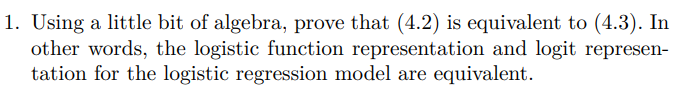
\includegraphics[width=1\textwidth,height=\textheight]{images/clipboard-4077728568.png}

}

\end{figure}

\begin{figure}

{\centering 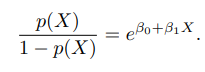
\includegraphics[width=0.4\textwidth,height=\textheight]{images/clipboard-3304908845.png}

}

\end{figure}

\begin{figure}

{\centering 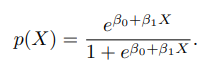
\includegraphics[width=0.4\textwidth,height=\textheight]{images/clipboard-249183538.png}

}

\end{figure}

\begin{center}\rule{0.5\linewidth}{0.5pt}\end{center}

Solution:

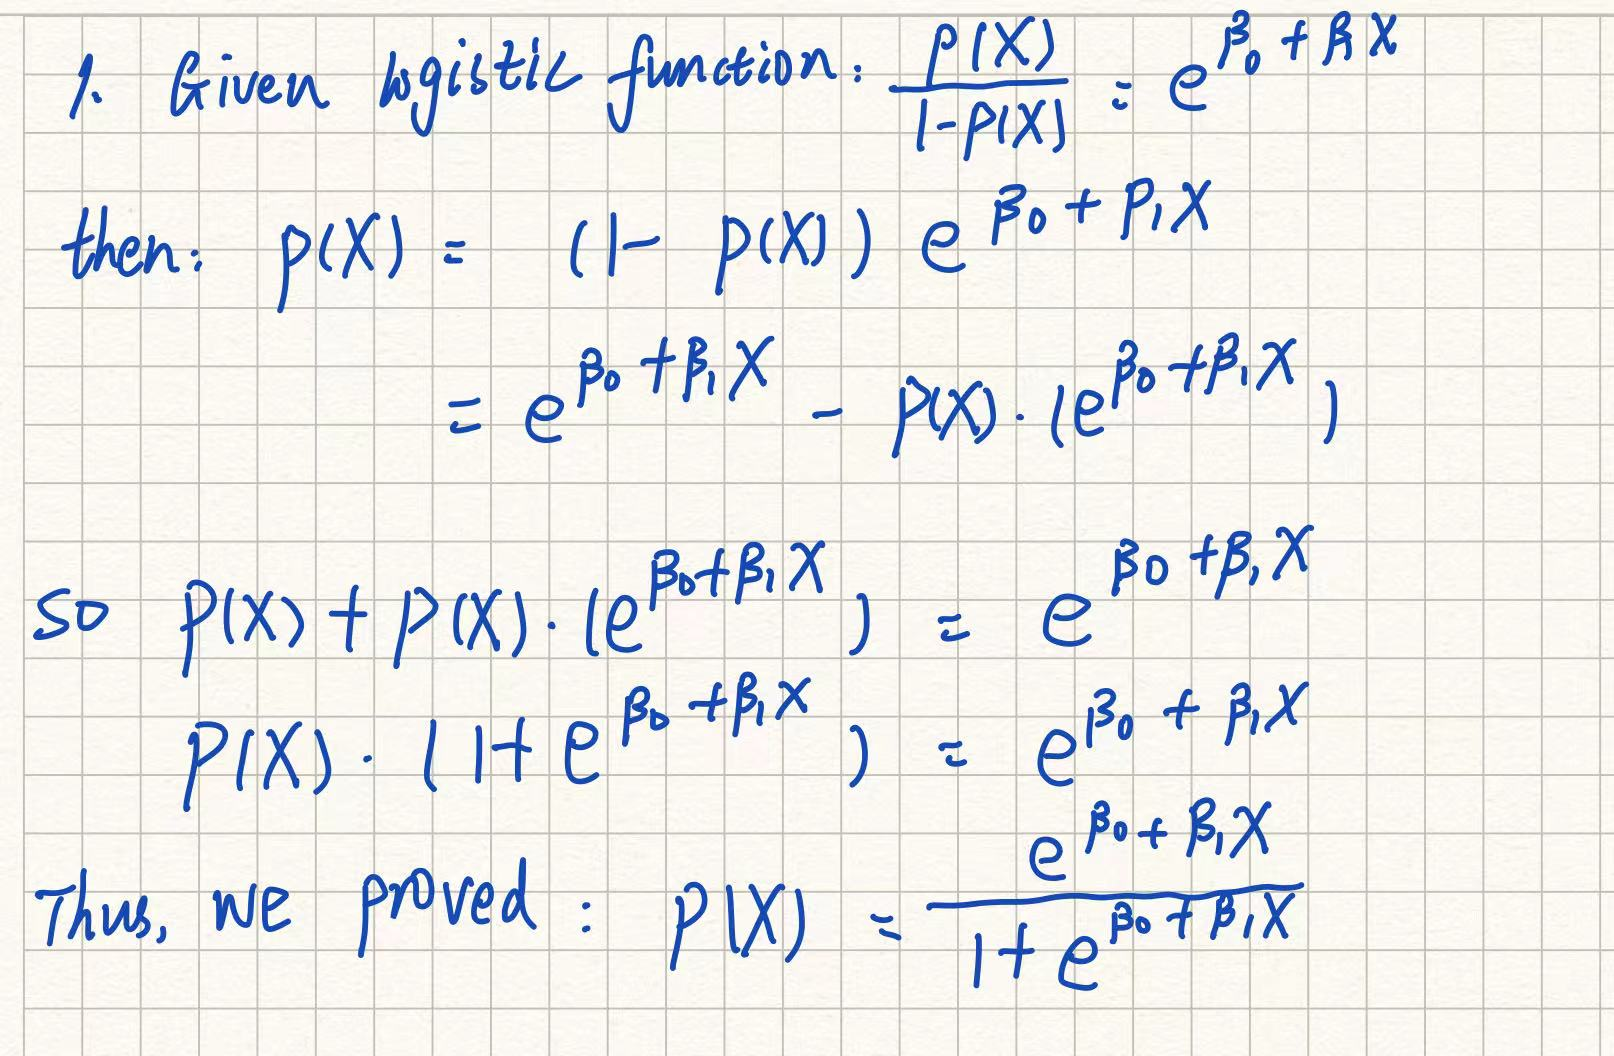
\includegraphics[width=6.875in,height=\textheight]{images/clipboard-2967000257.jpeg}

\hypertarget{isl-exercise-4.8.6-10pts}{%
\subsection{ISL Exercise 4.8.6 (10pts)}\label{isl-exercise-4.8.6-10pts}}

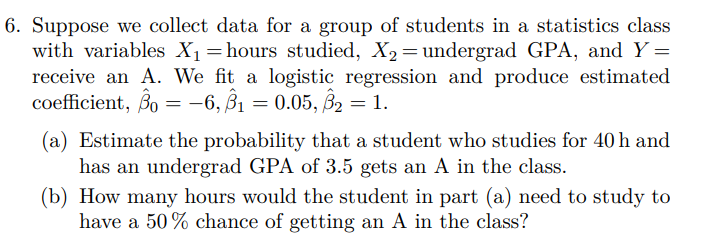
\includegraphics{images/clipboard-2695304714.png}

\begin{center}\rule{0.5\linewidth}{0.5pt}\end{center}

Solution:

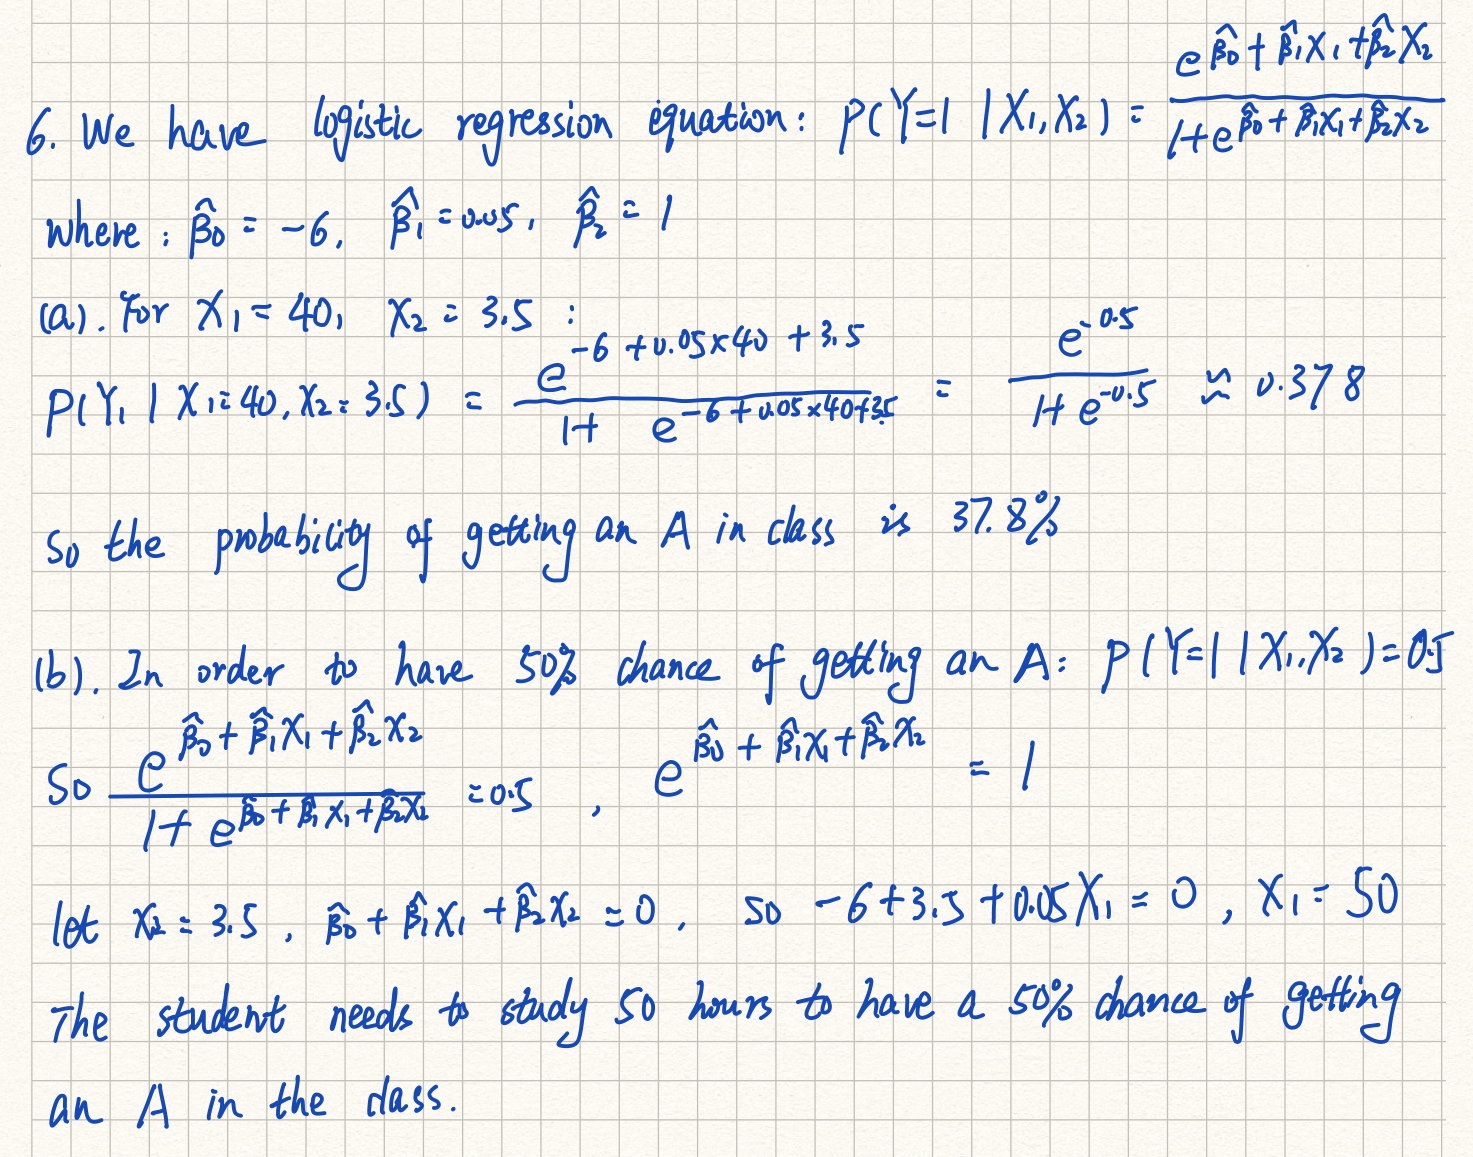
\includegraphics[width=6.9375in,height=\textheight]{images/clipboard-3585369922.jpeg}

\hypertarget{isl-exercise-4.8.9-10pts}{%
\subsection{ISL Exercise 4.8.9 (10pts)}\label{isl-exercise-4.8.9-10pts}}

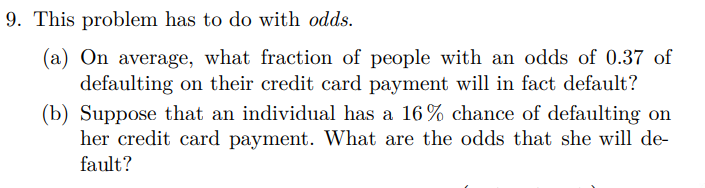
\includegraphics{images/clipboard-2955947930.png}

\begin{center}\rule{0.5\linewidth}{0.5pt}\end{center}

Solution:

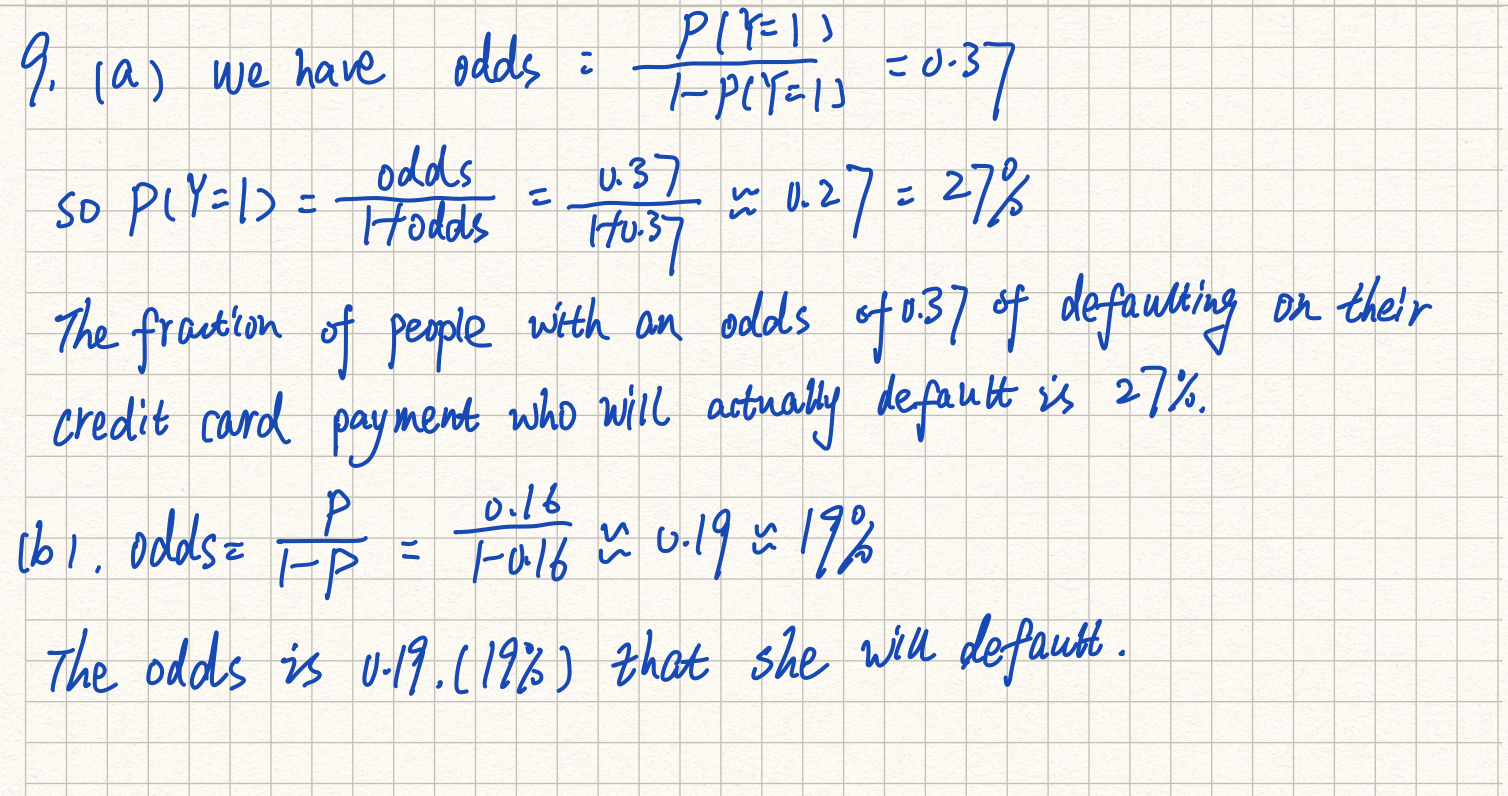
\includegraphics[width=7.03125in,height=\textheight]{images/clipboard-3451261091.jpeg}

\hypertarget{isl-exercise-4.8.13-a-i-50pts}{%
\subsection{ISL Exercise 4.8.13 (a)-(i)
(50pts)}\label{isl-exercise-4.8.13-a-i-50pts}}

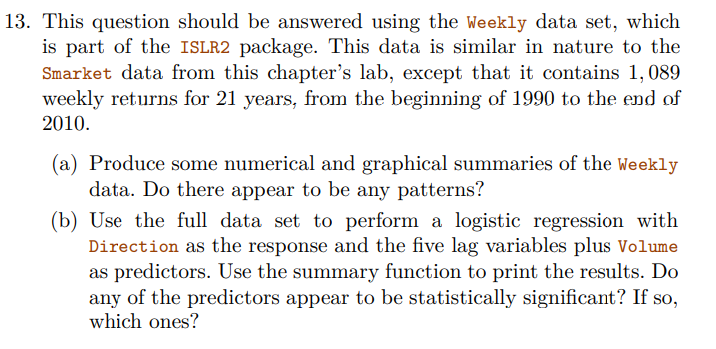
\includegraphics[width=6.94792in,height=\textheight]{images/clipboard-2962329981.png}

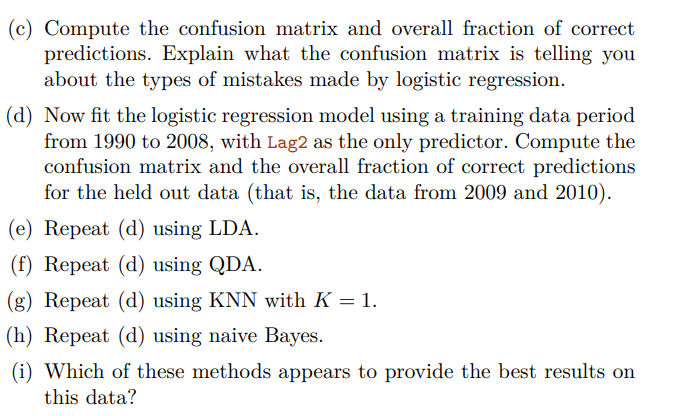
\includegraphics[width=6.88542in,height=\textheight]{images/clipboard-3390512393.png}

\begin{center}\rule{0.5\linewidth}{0.5pt}\end{center}

Solution:

\begin{Shaded}
\begin{Highlighting}[]
\FunctionTok{library}\NormalTok{(ISLR2)}
\FunctionTok{library}\NormalTok{(MASS)}

\FunctionTok{data}\NormalTok{(}\StringTok{"Weekly"}\NormalTok{)}
\CommentTok{\# Structure of the dataset}
\FunctionTok{str}\NormalTok{(Weekly)}
\end{Highlighting}
\end{Shaded}

\begin{verbatim}
'data.frame':   1089 obs. of  9 variables:
 $ Year     : num  1990 1990 1990 1990 1990 1990 1990 1990 1990 1990 ...
 $ Lag1     : num  0.816 -0.27 -2.576 3.514 0.712 ...
 $ Lag2     : num  1.572 0.816 -0.27 -2.576 3.514 ...
 $ Lag3     : num  -3.936 1.572 0.816 -0.27 -2.576 ...
 $ Lag4     : num  -0.229 -3.936 1.572 0.816 -0.27 ...
 $ Lag5     : num  -3.484 -0.229 -3.936 1.572 0.816 ...
 $ Volume   : num  0.155 0.149 0.16 0.162 0.154 ...
 $ Today    : num  -0.27 -2.576 3.514 0.712 1.178 ...
 $ Direction: Factor w/ 2 levels "Down","Up": 1 1 2 2 2 1 2 2 2 1 ...
\end{verbatim}

(a)

\begin{Shaded}
\begin{Highlighting}[]
\CommentTok{\# Numerical summary}
\FunctionTok{summary}\NormalTok{(Weekly)}
\end{Highlighting}
\end{Shaded}

\begin{verbatim}
      Year           Lag1               Lag2               Lag3         
 Min.   :1990   Min.   :-18.1950   Min.   :-18.1950   Min.   :-18.1950  
 1st Qu.:1995   1st Qu.: -1.1540   1st Qu.: -1.1540   1st Qu.: -1.1580  
 Median :2000   Median :  0.2410   Median :  0.2410   Median :  0.2410  
 Mean   :2000   Mean   :  0.1506   Mean   :  0.1511   Mean   :  0.1472  
 3rd Qu.:2005   3rd Qu.:  1.4050   3rd Qu.:  1.4090   3rd Qu.:  1.4090  
 Max.   :2010   Max.   : 12.0260   Max.   : 12.0260   Max.   : 12.0260  
      Lag4               Lag5              Volume            Today         
 Min.   :-18.1950   Min.   :-18.1950   Min.   :0.08747   Min.   :-18.1950  
 1st Qu.: -1.1580   1st Qu.: -1.1660   1st Qu.:0.33202   1st Qu.: -1.1540  
 Median :  0.2380   Median :  0.2340   Median :1.00268   Median :  0.2410  
 Mean   :  0.1458   Mean   :  0.1399   Mean   :1.57462   Mean   :  0.1499  
 3rd Qu.:  1.4090   3rd Qu.:  1.4050   3rd Qu.:2.05373   3rd Qu.:  1.4050  
 Max.   : 12.0260   Max.   : 12.0260   Max.   :9.32821   Max.   : 12.0260  
 Direction 
 Down:484  
 Up  :605  
           
           
           
           
\end{verbatim}

\begin{Shaded}
\begin{Highlighting}[]
\CommentTok{\# Plot the Volume over time}
\FunctionTok{plot}\NormalTok{(Weekly}\SpecialCharTok{$}\NormalTok{Year, Weekly}\SpecialCharTok{$}\NormalTok{Volume, }\AttributeTok{main=}\StringTok{"Trading Volume Over Time"}\NormalTok{, }\AttributeTok{xlab=}\StringTok{"Year"}\NormalTok{, }\AttributeTok{ylab=}\StringTok{"Volume"}\NormalTok{, }\AttributeTok{col=}\StringTok{"blue"}\NormalTok{, }\AttributeTok{pch=}\DecValTok{20}\NormalTok{)}
\end{Highlighting}
\end{Shaded}

\begin{figure}[H]

{\centering 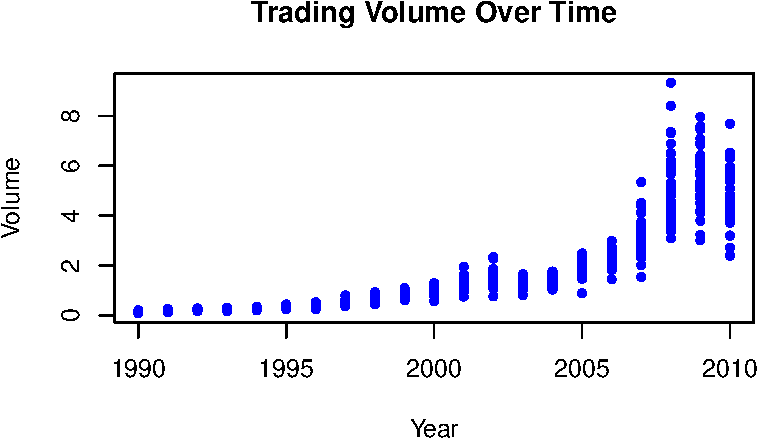
\includegraphics{hw2_files/figure-pdf/unnamed-chunk-4-1.pdf}

}

\end{figure}

\begin{Shaded}
\begin{Highlighting}[]
\CommentTok{\# Boxplot of market return (Today) by Direction}
\FunctionTok{boxplot}\NormalTok{(Today }\SpecialCharTok{\textasciitilde{}}\NormalTok{ Direction, }\AttributeTok{data=}\NormalTok{Weekly, }\AttributeTok{main=}\StringTok{"Market Return by Direction"}\NormalTok{, }\AttributeTok{ylab=}\StringTok{"Today’s Return"}\NormalTok{, }\AttributeTok{col=}\FunctionTok{c}\NormalTok{(}\StringTok{"red"}\NormalTok{, }\StringTok{"green"}\NormalTok{))}
\end{Highlighting}
\end{Shaded}

\begin{figure}[H]

{\centering 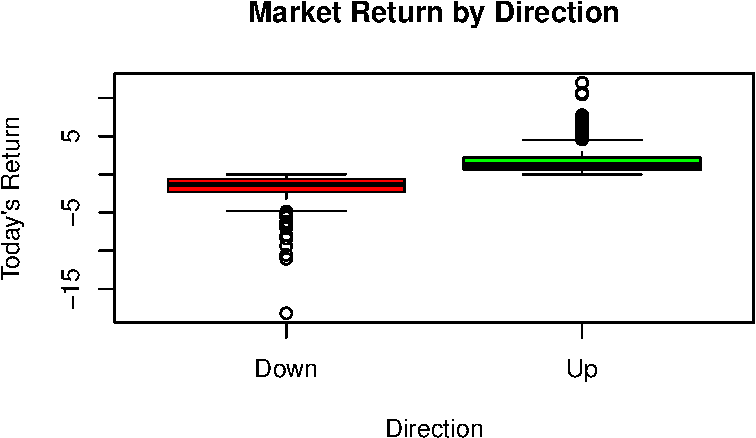
\includegraphics{hw2_files/figure-pdf/unnamed-chunk-4-2.pdf}

}

\end{figure}

\begin{Shaded}
\begin{Highlighting}[]
\CommentTok{\# Correlation matrix (excluding categorical variables)}
\FunctionTok{cor}\NormalTok{(Weekly[, }\SpecialCharTok{{-}}\DecValTok{9}\NormalTok{])  }\CommentTok{\# Exclude the Direction column}
\end{Highlighting}
\end{Shaded}

\begin{verbatim}
              Year         Lag1        Lag2        Lag3         Lag4
Year    1.00000000 -0.032289274 -0.03339001 -0.03000649 -0.031127923
Lag1   -0.03228927  1.000000000 -0.07485305  0.05863568 -0.071273876
Lag2   -0.03339001 -0.074853051  1.00000000 -0.07572091  0.058381535
Lag3   -0.03000649  0.058635682 -0.07572091  1.00000000 -0.075395865
Lag4   -0.03112792 -0.071273876  0.05838153 -0.07539587  1.000000000
Lag5   -0.03051910 -0.008183096 -0.07249948  0.06065717 -0.075675027
Volume  0.84194162 -0.064951313 -0.08551314 -0.06928771 -0.061074617
Today  -0.03245989 -0.075031842  0.05916672 -0.07124364 -0.007825873
               Lag5      Volume        Today
Year   -0.030519101  0.84194162 -0.032459894
Lag1   -0.008183096 -0.06495131 -0.075031842
Lag2   -0.072499482 -0.08551314  0.059166717
Lag3    0.060657175 -0.06928771 -0.071243639
Lag4   -0.075675027 -0.06107462 -0.007825873
Lag5    1.000000000 -0.05851741  0.011012698
Volume -0.058517414  1.00000000 -0.033077783
Today   0.011012698 -0.03307778  1.000000000
\end{verbatim}

Volume has increased significantly over time. Returns (Today) have a
mean near zero, indicating relatively balanced ups and downs in market
movement. The Direction variable (Up/Down) suggests a roughly even
split, meaning the market is not strongly biased in one direction.

Upward (Up) and downward (Down) movements have different distributions.
Down days have more extreme negative outliers, indicating higher risk
when the market declines. The median return is slightly higher for
``Up'' movements, but variance is similar for both.

(b)

\begin{Shaded}
\begin{Highlighting}[]
\CommentTok{\# Fit logistic regression model}
\NormalTok{logistic\_model }\OtherTok{\textless{}{-}} \FunctionTok{glm}\NormalTok{(Direction }\SpecialCharTok{\textasciitilde{}}\NormalTok{ Lag1 }\SpecialCharTok{+}\NormalTok{ Lag2 }\SpecialCharTok{+}\NormalTok{ Lag3 }\SpecialCharTok{+}\NormalTok{ Lag4 }\SpecialCharTok{+}\NormalTok{ Lag5 }\SpecialCharTok{+}\NormalTok{ Volume, }
                      \AttributeTok{data =}\NormalTok{ Weekly, }\AttributeTok{family =}\NormalTok{ binomial)}

\CommentTok{\# Summary of the logistic regression model}
\FunctionTok{summary}\NormalTok{(logistic\_model)}
\end{Highlighting}
\end{Shaded}

\begin{verbatim}

Call:
glm(formula = Direction ~ Lag1 + Lag2 + Lag3 + Lag4 + Lag5 + 
    Volume, family = binomial, data = Weekly)

Coefficients:
            Estimate Std. Error z value Pr(>|z|)   
(Intercept)  0.26686    0.08593   3.106   0.0019 **
Lag1        -0.04127    0.02641  -1.563   0.1181   
Lag2         0.05844    0.02686   2.175   0.0296 * 
Lag3        -0.01606    0.02666  -0.602   0.5469   
Lag4        -0.02779    0.02646  -1.050   0.2937   
Lag5        -0.01447    0.02638  -0.549   0.5833   
Volume      -0.02274    0.03690  -0.616   0.5377   
---
Signif. codes:  0 '***' 0.001 '**' 0.01 '*' 0.05 '.' 0.1 ' ' 1

(Dispersion parameter for binomial family taken to be 1)

    Null deviance: 1496.2  on 1088  degrees of freedom
Residual deviance: 1486.4  on 1082  degrees of freedom
AIC: 1500.4

Number of Fisher Scoring iterations: 4
\end{verbatim}

\(log(\frac{P(Up)}{1-P(Up)})\) = 0.26686−0.04127 × Lag1+0.05844 ×
Lag2−0.01066 × Lag3−0.02779 × Lag4−0.01447 × Lag5−0.02274 × Volume.

Yes, the p-values of Lag1 and Lag3 are less than 0.05, so they are
statistically significant.

(c)

\begin{Shaded}
\begin{Highlighting}[]
\CommentTok{\# Predict probabilities}
\NormalTok{pred\_probs }\OtherTok{\textless{}{-}} \FunctionTok{predict}\NormalTok{(logistic\_model, }\AttributeTok{type=}\StringTok{"response"}\NormalTok{)}

\CommentTok{\# Convert probabilities to class predictions (threshold = 0.5)}
\NormalTok{pred\_classes }\OtherTok{\textless{}{-}} \FunctionTok{ifelse}\NormalTok{(pred\_probs }\SpecialCharTok{\textgreater{}} \FloatTok{0.5}\NormalTok{, }\StringTok{"Up"}\NormalTok{, }\StringTok{"Down"}\NormalTok{)}

\CommentTok{\# Create confusion matrix}
\NormalTok{conf\_matrix }\OtherTok{\textless{}{-}} \FunctionTok{table}\NormalTok{(}\AttributeTok{Predicted =}\NormalTok{ pred\_classes, }\AttributeTok{Actual =}\NormalTok{ Weekly}\SpecialCharTok{$}\NormalTok{Direction)}

\CommentTok{\# Compute accuracy}
\NormalTok{accuracy }\OtherTok{\textless{}{-}} \FunctionTok{mean}\NormalTok{(pred\_classes }\SpecialCharTok{==}\NormalTok{ Weekly}\SpecialCharTok{$}\NormalTok{Direction)}

\CommentTok{\# Print results}
\FunctionTok{print}\NormalTok{(conf\_matrix)}
\end{Highlighting}
\end{Shaded}

\begin{verbatim}
         Actual
Predicted Down  Up
     Down   54  48
     Up    430 557
\end{verbatim}

\begin{Shaded}
\begin{Highlighting}[]
\FunctionTok{print}\NormalTok{(}\FunctionTok{paste}\NormalTok{(}\StringTok{"Overall accuracy:"}\NormalTok{, }\FunctionTok{round}\NormalTok{(accuracy, }\DecValTok{4}\NormalTok{)))}
\end{Highlighting}
\end{Shaded}

\begin{verbatim}
[1] "Overall accuracy: 0.5611"
\end{verbatim}

True Positives (TP) = 557 ; False Positives (FP) = 430 ; True Negatives
(TN) = 54 ; False Negatives (FN) = 48

Accuracy=
\(\frac{TP+TN}{Total Samples} = \frac{557+54}{54+48+430+557}=0.5611\) .
This is only slightly better than random guessing (50\%).

The model is biased towards predicting ``Up'', as indicated by the large
number of false positives (FP = 430). The model fails to predict
``Down'' accurately, with only 54 correct ``Down'' predictions out of
484 actual ``Down'' instances.

(d)

\begin{Shaded}
\begin{Highlighting}[]
\CommentTok{\# Split the dataset}
\NormalTok{train }\OtherTok{\textless{}{-}}\NormalTok{ Weekly}\SpecialCharTok{$}\NormalTok{Year }\SpecialCharTok{\textless{}} \DecValTok{2009}
\NormalTok{train\_data }\OtherTok{\textless{}{-}}\NormalTok{ Weekly[train, ]}
\NormalTok{test\_data }\OtherTok{\textless{}{-}}\NormalTok{ Weekly[}\SpecialCharTok{!}\NormalTok{train, ]}

\CommentTok{\# Fit logistic regression using Lag2}
\NormalTok{logistic\_model\_lag2 }\OtherTok{\textless{}{-}} \FunctionTok{glm}\NormalTok{(Direction }\SpecialCharTok{\textasciitilde{}}\NormalTok{ Lag2, }\AttributeTok{data=}\NormalTok{train\_data, }\AttributeTok{family=}\NormalTok{binomial)}

\CommentTok{\# Predict on test data}
\NormalTok{test\_probs }\OtherTok{\textless{}{-}} \FunctionTok{predict}\NormalTok{(logistic\_model\_lag2, }\AttributeTok{newdata=}\NormalTok{test\_data, }\AttributeTok{type=}\StringTok{"response"}\NormalTok{)}

\CommentTok{\# Convert probabilities to class labels}
\NormalTok{test\_preds }\OtherTok{\textless{}{-}} \FunctionTok{ifelse}\NormalTok{(test\_probs }\SpecialCharTok{\textgreater{}} \FloatTok{0.5}\NormalTok{, }\StringTok{"Up"}\NormalTok{, }\StringTok{"Down"}\NormalTok{)}

\CommentTok{\# Compute confusion matrix}
\NormalTok{conf\_matrix\_test }\OtherTok{\textless{}{-}} \FunctionTok{table}\NormalTok{(}\AttributeTok{Predicted =}\NormalTok{ test\_preds, }\AttributeTok{Actual =}\NormalTok{ test\_data}\SpecialCharTok{$}\NormalTok{Direction)}

\CommentTok{\# Compute accuracy}
\NormalTok{test\_accuracy }\OtherTok{\textless{}{-}} \FunctionTok{mean}\NormalTok{(test\_preds }\SpecialCharTok{==}\NormalTok{ test\_data}\SpecialCharTok{$}\NormalTok{Direction)}

\CommentTok{\# Print results}
\FunctionTok{print}\NormalTok{(conf\_matrix\_test)}
\end{Highlighting}
\end{Shaded}

\begin{verbatim}
         Actual
Predicted Down Up
     Down    9  5
     Up     34 56
\end{verbatim}

\begin{Shaded}
\begin{Highlighting}[]
\FunctionTok{print}\NormalTok{(}\FunctionTok{paste}\NormalTok{(}\StringTok{"Test accuracy:"}\NormalTok{, }\FunctionTok{round}\NormalTok{(test\_accuracy, }\DecValTok{4}\NormalTok{)))}
\end{Highlighting}
\end{Shaded}

\begin{verbatim}
[1] "Test accuracy: 0.625"
\end{verbatim}

(e)

\begin{Shaded}
\begin{Highlighting}[]
\CommentTok{\# Fit LDA model}
\NormalTok{lda\_model }\OtherTok{\textless{}{-}} \FunctionTok{lda}\NormalTok{(Direction }\SpecialCharTok{\textasciitilde{}}\NormalTok{ Lag2, }\AttributeTok{data=}\NormalTok{train\_data)}

\CommentTok{\# Predict on test data}
\NormalTok{lda\_preds }\OtherTok{\textless{}{-}} \FunctionTok{predict}\NormalTok{(lda\_model, }\AttributeTok{newdata=}\NormalTok{test\_data)}

\CommentTok{\# Extract class predictions}
\NormalTok{lda\_classes }\OtherTok{\textless{}{-}}\NormalTok{ lda\_preds}\SpecialCharTok{$}\NormalTok{class}

\CommentTok{\# Create confusion matrix}
\NormalTok{conf\_matrix\_lda }\OtherTok{\textless{}{-}} \FunctionTok{table}\NormalTok{(}\AttributeTok{Predicted =}\NormalTok{ lda\_classes, }\AttributeTok{Actual =}\NormalTok{ test\_data}\SpecialCharTok{$}\NormalTok{Direction)}

\CommentTok{\# Compute accuracy}
\NormalTok{lda\_accuracy }\OtherTok{\textless{}{-}} \FunctionTok{mean}\NormalTok{(lda\_classes }\SpecialCharTok{==}\NormalTok{ test\_data}\SpecialCharTok{$}\NormalTok{Direction)}

\CommentTok{\# Print results}
\FunctionTok{print}\NormalTok{(conf\_matrix\_lda)}
\end{Highlighting}
\end{Shaded}

\begin{verbatim}
         Actual
Predicted Down Up
     Down    9  5
     Up     34 56
\end{verbatim}

\begin{Shaded}
\begin{Highlighting}[]
\FunctionTok{print}\NormalTok{(}\FunctionTok{paste}\NormalTok{(}\StringTok{"LDA test accuracy:"}\NormalTok{, }\FunctionTok{round}\NormalTok{(lda\_accuracy, }\DecValTok{4}\NormalTok{)))}
\end{Highlighting}
\end{Shaded}

\begin{verbatim}
[1] "LDA test accuracy: 0.625"
\end{verbatim}

(f)

\begin{Shaded}
\begin{Highlighting}[]
\CommentTok{\# Fit QDA model}
\NormalTok{qda\_model }\OtherTok{\textless{}{-}} \FunctionTok{qda}\NormalTok{(Direction }\SpecialCharTok{\textasciitilde{}}\NormalTok{ Lag2, }\AttributeTok{data=}\NormalTok{train\_data)}

\CommentTok{\# Predict on test data}
\NormalTok{qda\_preds }\OtherTok{\textless{}{-}} \FunctionTok{predict}\NormalTok{(qda\_model, }\AttributeTok{newdata=}\NormalTok{test\_data)}

\CommentTok{\# Extract class predictions}
\NormalTok{qda\_classes }\OtherTok{\textless{}{-}}\NormalTok{ qda\_preds}\SpecialCharTok{$}\NormalTok{class}

\CommentTok{\# Compute confusion matrix}
\NormalTok{conf\_matrix\_qda }\OtherTok{\textless{}{-}} \FunctionTok{table}\NormalTok{(}\AttributeTok{Predicted =}\NormalTok{ qda\_classes, }\AttributeTok{Actual =}\NormalTok{ test\_data}\SpecialCharTok{$}\NormalTok{Direction)}

\CommentTok{\# Compute accuracy}
\NormalTok{qda\_accuracy }\OtherTok{\textless{}{-}} \FunctionTok{mean}\NormalTok{(qda\_classes }\SpecialCharTok{==}\NormalTok{ test\_data}\SpecialCharTok{$}\NormalTok{Direction)}

\CommentTok{\# Print results}
\FunctionTok{print}\NormalTok{(conf\_matrix\_qda)}
\end{Highlighting}
\end{Shaded}

\begin{verbatim}
         Actual
Predicted Down Up
     Down    0  0
     Up     43 61
\end{verbatim}

\begin{Shaded}
\begin{Highlighting}[]
\FunctionTok{print}\NormalTok{(}\FunctionTok{paste}\NormalTok{(}\StringTok{"QDA test accuracy:"}\NormalTok{, }\FunctionTok{round}\NormalTok{(qda\_accuracy, }\DecValTok{4}\NormalTok{)))}
\end{Highlighting}
\end{Shaded}

\begin{verbatim}
[1] "QDA test accuracy: 0.5865"
\end{verbatim}

(g)

\begin{Shaded}
\begin{Highlighting}[]
\FunctionTok{library}\NormalTok{(class)}

\CommentTok{\# Prepare training and test data}
\NormalTok{train\_X }\OtherTok{\textless{}{-}}\NormalTok{ train\_data}\SpecialCharTok{$}\NormalTok{Lag2}
\NormalTok{test\_X }\OtherTok{\textless{}{-}}\NormalTok{ test\_data}\SpecialCharTok{$}\NormalTok{Lag2}
\NormalTok{train\_Y }\OtherTok{\textless{}{-}}\NormalTok{ train\_data}\SpecialCharTok{$}\NormalTok{Direction}
\NormalTok{test\_Y }\OtherTok{\textless{}{-}}\NormalTok{ test\_data}\SpecialCharTok{$}\NormalTok{Direction}

\CommentTok{\# Apply KNN with K=1}
\NormalTok{knn\_preds }\OtherTok{\textless{}{-}} \FunctionTok{knn}\NormalTok{(}\AttributeTok{train =} \FunctionTok{matrix}\NormalTok{(train\_X), }\AttributeTok{test =} \FunctionTok{matrix}\NormalTok{(test\_X), }
                 \AttributeTok{cl =}\NormalTok{ train\_Y, }\AttributeTok{k =} \DecValTok{1}\NormalTok{)}

\CommentTok{\# Compute confusion matrix}
\NormalTok{conf\_matrix\_knn }\OtherTok{\textless{}{-}} \FunctionTok{table}\NormalTok{(}\AttributeTok{Predicted =}\NormalTok{ knn\_preds, }\AttributeTok{Actual =}\NormalTok{ test\_Y)}

\CommentTok{\# Compute accuracy}
\NormalTok{knn\_accuracy }\OtherTok{\textless{}{-}} \FunctionTok{mean}\NormalTok{(knn\_preds }\SpecialCharTok{==}\NormalTok{ test\_Y)}

\CommentTok{\# Print results}
\FunctionTok{print}\NormalTok{(conf\_matrix\_knn)}
\end{Highlighting}
\end{Shaded}

\begin{verbatim}
         Actual
Predicted Down Up
     Down   21 30
     Up     22 31
\end{verbatim}

\begin{Shaded}
\begin{Highlighting}[]
\FunctionTok{print}\NormalTok{(}\FunctionTok{paste}\NormalTok{(}\StringTok{"KNN (K=1) test accuracy:"}\NormalTok{, }\FunctionTok{round}\NormalTok{(knn\_accuracy, }\DecValTok{4}\NormalTok{)))}
\end{Highlighting}
\end{Shaded}

\begin{verbatim}
[1] "KNN (K=1) test accuracy: 0.5"
\end{verbatim}

(h)

\begin{Shaded}
\begin{Highlighting}[]
\FunctionTok{library}\NormalTok{(e1071)}

\CommentTok{\# Fit Naive Bayes model}
\NormalTok{nb\_model }\OtherTok{\textless{}{-}} \FunctionTok{naiveBayes}\NormalTok{(Direction }\SpecialCharTok{\textasciitilde{}}\NormalTok{ Lag2, }\AttributeTok{data=}\NormalTok{train\_data)}

\CommentTok{\# Predict on test data}
\NormalTok{nb\_preds }\OtherTok{\textless{}{-}} \FunctionTok{predict}\NormalTok{(nb\_model, }\AttributeTok{newdata=}\NormalTok{test\_data)}

\CommentTok{\# Compute confusion matrix}
\NormalTok{conf\_matrix\_nb }\OtherTok{\textless{}{-}} \FunctionTok{table}\NormalTok{(}\AttributeTok{Predicted =}\NormalTok{ nb\_preds, }\AttributeTok{Actual =}\NormalTok{ test\_data}\SpecialCharTok{$}\NormalTok{Direction)}

\CommentTok{\# Compute accuracy}
\NormalTok{nb\_accuracy }\OtherTok{\textless{}{-}} \FunctionTok{mean}\NormalTok{(nb\_preds }\SpecialCharTok{==}\NormalTok{ test\_data}\SpecialCharTok{$}\NormalTok{Direction)}

\CommentTok{\# Print results}
\FunctionTok{print}\NormalTok{(conf\_matrix\_nb)}
\end{Highlighting}
\end{Shaded}

\begin{verbatim}
         Actual
Predicted Down Up
     Down    0  0
     Up     43 61
\end{verbatim}

\begin{Shaded}
\begin{Highlighting}[]
\FunctionTok{print}\NormalTok{(}\FunctionTok{paste}\NormalTok{(}\StringTok{"Naive Bayes test accuracy:"}\NormalTok{, }\FunctionTok{round}\NormalTok{(nb\_accuracy, }\DecValTok{4}\NormalTok{)))}
\end{Highlighting}
\end{Shaded}

\begin{verbatim}
[1] "Naive Bayes test accuracy: 0.5865"
\end{verbatim}

(i)

\begin{Shaded}
\begin{Highlighting}[]
\CommentTok{\# Create a comparison table}
\NormalTok{model\_comparison }\OtherTok{\textless{}{-}} \FunctionTok{data.frame}\NormalTok{(}
  \AttributeTok{Model =} \FunctionTok{c}\NormalTok{(}\StringTok{"Logistic Regression"}\NormalTok{, }\StringTok{"LDA"}\NormalTok{, }\StringTok{"QDA"}\NormalTok{, }\StringTok{"KNN (K=1)"}\NormalTok{, }
            \StringTok{"Naive Bayes"}\NormalTok{),}
  \AttributeTok{Accuracy =} \FunctionTok{c}\NormalTok{(test\_accuracy, lda\_accuracy, qda\_accuracy, }
\NormalTok{               knn\_accuracy, nb\_accuracy)}
\NormalTok{)}

\CommentTok{\# Print comparison results}
\FunctionTok{print}\NormalTok{(model\_comparison)}
\end{Highlighting}
\end{Shaded}

\begin{verbatim}
                Model  Accuracy
1 Logistic Regression 0.6250000
2                 LDA 0.6250000
3                 QDA 0.5865385
4           KNN (K=1) 0.5000000
5         Naive Bayes 0.5865385
\end{verbatim}

The Logistic Regression and LDA appear to have the best results on this
data, and they both have 0.625 accuracy.

\hypertarget{bonus-question-isl-exercise-4.8.13-part-j-30pts}{%
\subsection{Bonus question: ISL Exercise 4.8.13 Part (j)
(30pts)}\label{bonus-question-isl-exercise-4.8.13-part-j-30pts}}

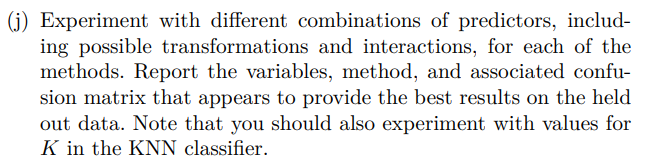
\includegraphics{images/clipboard-698312542.png}

\begin{center}\rule{0.5\linewidth}{0.5pt}\end{center}

Solution:

(j) Logistic Regression with multiple predictors

\begin{Shaded}
\begin{Highlighting}[]
\NormalTok{logistic\_model\_extended }\OtherTok{\textless{}{-}} \FunctionTok{glm}\NormalTok{(Direction }\SpecialCharTok{\textasciitilde{}}\NormalTok{ Lag1 }\SpecialCharTok{+}\NormalTok{ Lag2 }\SpecialCharTok{+}\NormalTok{ Lag3 }\SpecialCharTok{+}\NormalTok{ Lag4 }\SpecialCharTok{+}\NormalTok{ Lag5 }\SpecialCharTok{+}\NormalTok{ Volume, }
                               \AttributeTok{data=}\NormalTok{train\_data, }\AttributeTok{family=}\NormalTok{binomial)}

\CommentTok{\# Predictions}
\NormalTok{test\_probs\_extended }\OtherTok{\textless{}{-}} \FunctionTok{predict}\NormalTok{(logistic\_model\_extended, }\AttributeTok{newdata=}\NormalTok{test\_data, }\AttributeTok{type=}\StringTok{"response"}\NormalTok{)}
\NormalTok{test\_preds\_extended }\OtherTok{\textless{}{-}} \FunctionTok{ifelse}\NormalTok{(test\_probs\_extended }\SpecialCharTok{\textgreater{}} \FloatTok{0.5}\NormalTok{, }\StringTok{"Up"}\NormalTok{, }\StringTok{"Down"}\NormalTok{)}

\CommentTok{\# Confusion Matrix}
\NormalTok{conf\_matrix\_logistic\_extended }\OtherTok{\textless{}{-}} \FunctionTok{table}\NormalTok{(}\AttributeTok{Predicted =}\NormalTok{ test\_preds\_extended, }\AttributeTok{Actual =}\NormalTok{ test\_data}\SpecialCharTok{$}\NormalTok{Direction)}
\NormalTok{logistic\_accuracy\_extended }\OtherTok{\textless{}{-}} \FunctionTok{mean}\NormalTok{(test\_preds\_extended }\SpecialCharTok{==}\NormalTok{ test\_data}\SpecialCharTok{$}\NormalTok{Direction)}

\FunctionTok{print}\NormalTok{(conf\_matrix\_logistic\_extended)}
\end{Highlighting}
\end{Shaded}

\begin{verbatim}
         Actual
Predicted Down Up
     Down   31 44
     Up     12 17
\end{verbatim}

\begin{Shaded}
\begin{Highlighting}[]
\FunctionTok{print}\NormalTok{(}\FunctionTok{paste}\NormalTok{(}\StringTok{"Extended Logistic Regression Accuracy:"}\NormalTok{, }\FunctionTok{round}\NormalTok{(logistic\_accuracy\_extended, }\DecValTok{4}\NormalTok{)))}
\end{Highlighting}
\end{Shaded}

\begin{verbatim}
[1] "Extended Logistic Regression Accuracy: 0.4615"
\end{verbatim}

Logistic Regression with interaction terms

\begin{Shaded}
\begin{Highlighting}[]
\NormalTok{logistic\_model\_interaction }\OtherTok{\textless{}{-}} \FunctionTok{glm}\NormalTok{(Direction }\SpecialCharTok{\textasciitilde{}}\NormalTok{ Lag2 }\SpecialCharTok{*}\NormalTok{ Volume, }
                                  \AttributeTok{data=}\NormalTok{train\_data, }\AttributeTok{family=}\NormalTok{binomial)}

\CommentTok{\# Predictions}
\NormalTok{test\_probs\_interaction }\OtherTok{\textless{}{-}} \FunctionTok{predict}\NormalTok{(logistic\_model\_interaction, }
                                  \AttributeTok{newdata=}\NormalTok{test\_data, }\AttributeTok{type=}\StringTok{"response"}\NormalTok{)}
\NormalTok{test\_preds\_interaction }\OtherTok{\textless{}{-}} \FunctionTok{ifelse}\NormalTok{(test\_probs\_interaction }\SpecialCharTok{\textgreater{}} \FloatTok{0.5}\NormalTok{, }\StringTok{"Up"}\NormalTok{, }\StringTok{"Down"}\NormalTok{)}

\CommentTok{\# Confusion Matrix}
\NormalTok{conf\_matrix\_logistic\_interaction }\OtherTok{\textless{}{-}} \FunctionTok{table}\NormalTok{(}\AttributeTok{Predicted =}\NormalTok{ test\_preds\_interaction, }
                                          \AttributeTok{Actual =}\NormalTok{ test\_data}\SpecialCharTok{$}\NormalTok{Direction)}
\NormalTok{logistic\_accuracy\_interaction }\OtherTok{\textless{}{-}} \FunctionTok{mean}\NormalTok{(}
\NormalTok{  test\_preds\_interaction }\SpecialCharTok{==}\NormalTok{ test\_data}\SpecialCharTok{$}\NormalTok{Direction}
\NormalTok{  )}

\FunctionTok{print}\NormalTok{(conf\_matrix\_logistic\_interaction)}
\end{Highlighting}
\end{Shaded}

\begin{verbatim}
         Actual
Predicted Down Up
     Down   20 25
     Up     23 36
\end{verbatim}

\begin{Shaded}
\begin{Highlighting}[]
\FunctionTok{print}\NormalTok{(}\FunctionTok{paste}\NormalTok{(}\StringTok{"Logistic Regression with Interaction Accuracy:"}\NormalTok{, }
            \FunctionTok{round}\NormalTok{(logistic\_accuracy\_interaction, }\DecValTok{4}\NormalTok{)))}
\end{Highlighting}
\end{Shaded}

\begin{verbatim}
[1] "Logistic Regression with Interaction Accuracy: 0.5385"
\end{verbatim}

LDA with More Predictors

\begin{Shaded}
\begin{Highlighting}[]
\FunctionTok{library}\NormalTok{(MASS)}
\NormalTok{lda\_model\_extended }\OtherTok{\textless{}{-}} \FunctionTok{lda}\NormalTok{(Direction }\SpecialCharTok{\textasciitilde{}}\NormalTok{ Lag1 }\SpecialCharTok{+}\NormalTok{ Lag2 }\SpecialCharTok{+}\NormalTok{ Lag3 }\SpecialCharTok{+}\NormalTok{ Lag4 }\SpecialCharTok{+}\NormalTok{ Lag5 }\SpecialCharTok{+}\NormalTok{ Volume, }
                          \AttributeTok{data=}\NormalTok{train\_data)}

\CommentTok{\# Predictions}
\NormalTok{lda\_preds\_extended }\OtherTok{\textless{}{-}} \FunctionTok{predict}\NormalTok{(lda\_model\_extended, }\AttributeTok{newdata=}\NormalTok{test\_data)}\SpecialCharTok{$}\NormalTok{class}

\CommentTok{\# Confusion Matrix}
\NormalTok{conf\_matrix\_lda\_extended }\OtherTok{\textless{}{-}} \FunctionTok{table}\NormalTok{(}\AttributeTok{Predicted =}\NormalTok{ lda\_preds\_extended, }\AttributeTok{Actual =} 
\NormalTok{                                    test\_data}\SpecialCharTok{$}\NormalTok{Direction)}
\NormalTok{lda\_accuracy\_extended }\OtherTok{\textless{}{-}} \FunctionTok{mean}\NormalTok{(lda\_preds\_extended }\SpecialCharTok{==}\NormalTok{ test\_data}\SpecialCharTok{$}\NormalTok{Direction)}

\FunctionTok{print}\NormalTok{(conf\_matrix\_lda\_extended)}
\end{Highlighting}
\end{Shaded}

\begin{verbatim}
         Actual
Predicted Down Up
     Down   31 44
     Up     12 17
\end{verbatim}

\begin{Shaded}
\begin{Highlighting}[]
\FunctionTok{print}\NormalTok{(}\FunctionTok{paste}\NormalTok{(}\StringTok{"Extended LDA Accuracy:"}\NormalTok{, }\FunctionTok{round}\NormalTok{(lda\_accuracy\_extended, }\DecValTok{4}\NormalTok{)))}
\end{Highlighting}
\end{Shaded}

\begin{verbatim}
[1] "Extended LDA Accuracy: 0.4615"
\end{verbatim}

QDA with More Predictors

\begin{Shaded}
\begin{Highlighting}[]
\NormalTok{qda\_model\_extended }\OtherTok{\textless{}{-}} \FunctionTok{qda}\NormalTok{(Direction }\SpecialCharTok{\textasciitilde{}}\NormalTok{ Lag1 }\SpecialCharTok{+}\NormalTok{ Lag2 }\SpecialCharTok{+}\NormalTok{ Lag3 }\SpecialCharTok{+}\NormalTok{ Lag4 }\SpecialCharTok{+}\NormalTok{ Lag5 }\SpecialCharTok{+}\NormalTok{ Volume, }
                          \AttributeTok{data=}\NormalTok{train\_data)}

\CommentTok{\# Predictions}
\NormalTok{qda\_preds\_extended }\OtherTok{\textless{}{-}} \FunctionTok{predict}\NormalTok{(qda\_model\_extended, }\AttributeTok{newdata=}\NormalTok{test\_data)}\SpecialCharTok{$}\NormalTok{class}

\CommentTok{\# Confusion Matrix}
\NormalTok{conf\_matrix\_qda\_extended }\OtherTok{\textless{}{-}} \FunctionTok{table}\NormalTok{(}\AttributeTok{Predicted =}\NormalTok{ qda\_preds\_extended, }\AttributeTok{Actual =} 
\NormalTok{                                    test\_data}\SpecialCharTok{$}\NormalTok{Direction)}
\NormalTok{qda\_accuracy\_extended }\OtherTok{\textless{}{-}} \FunctionTok{mean}\NormalTok{(qda\_preds\_extended }\SpecialCharTok{==}\NormalTok{ test\_data}\SpecialCharTok{$}\NormalTok{Direction)}

\FunctionTok{print}\NormalTok{(conf\_matrix\_qda\_extended)}
\end{Highlighting}
\end{Shaded}

\begin{verbatim}
         Actual
Predicted Down Up
     Down   33 49
     Up     10 12
\end{verbatim}

\begin{Shaded}
\begin{Highlighting}[]
\FunctionTok{print}\NormalTok{(}\FunctionTok{paste}\NormalTok{(}\StringTok{"Extended QDA Accuracy:"}\NormalTok{, }\FunctionTok{round}\NormalTok{(qda\_accuracy\_extended, }\DecValTok{4}\NormalTok{)))}
\end{Highlighting}
\end{Shaded}

\begin{verbatim}
[1] "Extended QDA Accuracy: 0.4327"
\end{verbatim}

Tuning K for KNN

\begin{Shaded}
\begin{Highlighting}[]
\FunctionTok{library}\NormalTok{(class)}

\CommentTok{\# Function to evaluate KNN for different K values}
\NormalTok{knn\_evaluate }\OtherTok{\textless{}{-}} \ControlFlowTok{function}\NormalTok{(k) \{}
\NormalTok{  knn\_preds }\OtherTok{\textless{}{-}} \FunctionTok{knn}\NormalTok{(}\AttributeTok{train=}\FunctionTok{as.matrix}\NormalTok{(train\_data[, }\FunctionTok{c}\NormalTok{(}\StringTok{"Lag2"}\NormalTok{)]), }
                   \AttributeTok{test=}\FunctionTok{as.matrix}\NormalTok{(test\_data[, }\FunctionTok{c}\NormalTok{(}\StringTok{"Lag2"}\NormalTok{)]), }
                   \AttributeTok{cl=}\NormalTok{train\_data}\SpecialCharTok{$}\NormalTok{Direction, }\AttributeTok{k=}\NormalTok{k)}
  
\NormalTok{  conf\_matrix\_knn }\OtherTok{\textless{}{-}} \FunctionTok{table}\NormalTok{(}\AttributeTok{Predicted =}\NormalTok{ knn\_preds, }\AttributeTok{Actual =}\NormalTok{ test\_data}\SpecialCharTok{$}\NormalTok{Direction)}
\NormalTok{  knn\_accuracy }\OtherTok{\textless{}{-}} \FunctionTok{mean}\NormalTok{(knn\_preds }\SpecialCharTok{==}\NormalTok{ test\_data}\SpecialCharTok{$}\NormalTok{Direction)}
  
  \FunctionTok{return}\NormalTok{(}\FunctionTok{list}\NormalTok{(}\AttributeTok{conf\_matrix=}\NormalTok{conf\_matrix\_knn, }\AttributeTok{accuracy=}\NormalTok{knn\_accuracy))}
\NormalTok{\}}

\CommentTok{\# Experiment with different values of K}
\NormalTok{knn\_results }\OtherTok{\textless{}{-}} \FunctionTok{lapply}\NormalTok{(}\FunctionTok{c}\NormalTok{(}\DecValTok{1}\NormalTok{, }\DecValTok{3}\NormalTok{, }\DecValTok{5}\NormalTok{, }\DecValTok{7}\NormalTok{, }\DecValTok{10}\NormalTok{, }\DecValTok{15}\NormalTok{, }\DecValTok{20}\NormalTok{), knn\_evaluate)}

\CommentTok{\# Print results for each K}
\ControlFlowTok{for}\NormalTok{ (i }\ControlFlowTok{in} \DecValTok{1}\SpecialCharTok{:}\FunctionTok{length}\NormalTok{(knn\_results)) \{}
  \FunctionTok{print}\NormalTok{(}\FunctionTok{paste}\NormalTok{(}\StringTok{"KNN with K ="}\NormalTok{, }\FunctionTok{c}\NormalTok{(}\DecValTok{1}\NormalTok{, }\DecValTok{3}\NormalTok{, }\DecValTok{5}\NormalTok{, }\DecValTok{7}\NormalTok{, }\DecValTok{10}\NormalTok{, }\DecValTok{15}\NormalTok{, }\DecValTok{20}\NormalTok{)[i]))}
  \FunctionTok{print}\NormalTok{(knn\_results[[i]]}\SpecialCharTok{$}\NormalTok{conf\_matrix)}
  \FunctionTok{print}\NormalTok{(}\FunctionTok{paste}\NormalTok{(}\StringTok{"Accuracy:"}\NormalTok{, }\FunctionTok{round}\NormalTok{(knn\_results[[i]]}\SpecialCharTok{$}\NormalTok{accuracy, }\DecValTok{4}\NormalTok{)))}
\NormalTok{\}}
\end{Highlighting}
\end{Shaded}

\begin{verbatim}
[1] "KNN with K = 1"
         Actual
Predicted Down Up
     Down   21 30
     Up     22 31
[1] "Accuracy: 0.5"
[1] "KNN with K = 3"
         Actual
Predicted Down Up
     Down   15 19
     Up     28 42
[1] "Accuracy: 0.5481"
[1] "KNN with K = 5"
         Actual
Predicted Down Up
     Down   15 21
     Up     28 40
[1] "Accuracy: 0.5288"
[1] "KNN with K = 7"
         Actual
Predicted Down Up
     Down   15 20
     Up     28 41
[1] "Accuracy: 0.5385"
[1] "KNN with K = 10"
         Actual
Predicted Down Up
     Down   17 19
     Up     26 42
[1] "Accuracy: 0.5673"
[1] "KNN with K = 15"
         Actual
Predicted Down Up
     Down   20 20
     Up     23 41
[1] "Accuracy: 0.5865"
[1] "KNN with K = 20"
         Actual
Predicted Down Up
     Down   20 20
     Up     23 41
[1] "Accuracy: 0.5865"
\end{verbatim}

Naive Bayes with More Predictors

\begin{Shaded}
\begin{Highlighting}[]
\FunctionTok{library}\NormalTok{(e1071)}
\NormalTok{nb\_model\_extended }\OtherTok{\textless{}{-}} \FunctionTok{naiveBayes}\NormalTok{(Direction }\SpecialCharTok{\textasciitilde{}}\NormalTok{ Lag1 }\SpecialCharTok{+}\NormalTok{ Lag2 }\SpecialCharTok{+} 
\NormalTok{                                  Lag3 }\SpecialCharTok{+}\NormalTok{ Lag4 }\SpecialCharTok{+}\NormalTok{ Lag5 }\SpecialCharTok{+}\NormalTok{ Volume, }\AttributeTok{data=}\NormalTok{train\_data)}

\CommentTok{\# Predictions}
\NormalTok{nb\_preds\_extended }\OtherTok{\textless{}{-}} \FunctionTok{predict}\NormalTok{(nb\_model\_extended, }\AttributeTok{newdata=}\NormalTok{test\_data)}

\CommentTok{\# Confusion Matrix}
\NormalTok{conf\_matrix\_nb\_extended }\OtherTok{\textless{}{-}} \FunctionTok{table}\NormalTok{(}\AttributeTok{Predicted =}\NormalTok{ nb\_preds\_extended, }\AttributeTok{Actual =} 
\NormalTok{                                   test\_data}\SpecialCharTok{$}\NormalTok{Direction)}
\NormalTok{nb\_accuracy\_extended }\OtherTok{\textless{}{-}} \FunctionTok{mean}\NormalTok{(nb\_preds\_extended }\SpecialCharTok{==}\NormalTok{ test\_data}\SpecialCharTok{$}\NormalTok{Direction)}

\FunctionTok{print}\NormalTok{(conf\_matrix\_nb\_extended)}
\end{Highlighting}
\end{Shaded}

\begin{verbatim}
         Actual
Predicted Down Up
     Down   42 56
     Up      1  5
\end{verbatim}

\begin{Shaded}
\begin{Highlighting}[]
\FunctionTok{print}\NormalTok{(}\FunctionTok{paste}\NormalTok{(}\StringTok{"Extended Naive Bayes Accuracy:"}\NormalTok{, }\FunctionTok{round}\NormalTok{(nb\_accuracy\_extended, }\DecValTok{4}\NormalTok{)))}
\end{Highlighting}
\end{Shaded}

\begin{verbatim}
[1] "Extended Naive Bayes Accuracy: 0.4519"
\end{verbatim}

Comparing All Models

\begin{Shaded}
\begin{Highlighting}[]
\CommentTok{\# Create a comparison table}
\NormalTok{model\_comparison }\OtherTok{\textless{}{-}} \FunctionTok{data.frame}\NormalTok{(}
  \AttributeTok{Model =} \FunctionTok{c}\NormalTok{(}\StringTok{"Logistic Regression"}\NormalTok{, }\StringTok{"logistic\_model\_extended"}\NormalTok{, }
            \StringTok{"Logistic Regression (Interaction)"}\NormalTok{, }
            \StringTok{"LDA"}\NormalTok{, }\StringTok{"LDA (Extended)"}\NormalTok{, }\StringTok{"QDA"}\NormalTok{, }\StringTok{"QDA (Extended)"}\NormalTok{, }
            \StringTok{"KNN (K=1)"}\NormalTok{,}\StringTok{"KNN (K=3)"}\NormalTok{, }\StringTok{"KNN (K=5)"}\NormalTok{, }\StringTok{"KNN (K=7)"}\NormalTok{, }
            \StringTok{"KNN (K=10)"}\NormalTok{, }\StringTok{"KNN (K=15)"}\NormalTok{, }\StringTok{"KNN (K=20)"}\NormalTok{, }
            \StringTok{"Naive Bayes"}\NormalTok{, }\StringTok{"Naive Bayes (Extended)"}\NormalTok{),}
  \AttributeTok{Accuracy =} \FunctionTok{c}\NormalTok{(test\_accuracy, logistic\_accuracy\_extended, }
\NormalTok{               logistic\_accuracy\_interaction, }
\NormalTok{               lda\_accuracy, lda\_accuracy\_extended, }
\NormalTok{               qda\_accuracy, qda\_accuracy\_extended, }
\NormalTok{               knn\_results[[}\DecValTok{1}\NormalTok{]]}\SpecialCharTok{$}\NormalTok{accuracy, knn\_results[[}\DecValTok{2}\NormalTok{]]}\SpecialCharTok{$}\NormalTok{accuracy, }
\NormalTok{               knn\_results[[}\DecValTok{3}\NormalTok{]]}\SpecialCharTok{$}\NormalTok{accuracy, knn\_results[[}\DecValTok{4}\NormalTok{]]}\SpecialCharTok{$}\NormalTok{accuracy, }
\NormalTok{               knn\_results[[}\DecValTok{5}\NormalTok{]]}\SpecialCharTok{$}\NormalTok{accuracy, knn\_results[[}\DecValTok{6}\NormalTok{]]}\SpecialCharTok{$}\NormalTok{accuracy, }
\NormalTok{               knn\_results[[}\DecValTok{7}\NormalTok{]]}\SpecialCharTok{$}\NormalTok{accuracy,}
\NormalTok{               nb\_accuracy, nb\_accuracy\_extended)}
\NormalTok{)}

\CommentTok{\# Print comparison results}
\FunctionTok{print}\NormalTok{(model\_comparison)}
\end{Highlighting}
\end{Shaded}

\begin{verbatim}
                               Model  Accuracy
1                Logistic Regression 0.6250000
2            logistic_model_extended 0.4615385
3  Logistic Regression (Interaction) 0.5384615
4                                LDA 0.6250000
5                     LDA (Extended) 0.4615385
6                                QDA 0.5865385
7                     QDA (Extended) 0.4326923
8                          KNN (K=1) 0.5000000
9                          KNN (K=3) 0.5480769
10                         KNN (K=5) 0.5288462
11                         KNN (K=7) 0.5384615
12                        KNN (K=10) 0.5673077
13                        KNN (K=15) 0.5865385
14                        KNN (K=20) 0.5865385
15                       Naive Bayes 0.5865385
16            Naive Bayes (Extended) 0.4519231
\end{verbatim}

\hypertarget{bonus-question-isl-exercise-4.8.4-30pts}{%
\subsection{Bonus question: ISL Exercise 4.8.4
(30pts)}\label{bonus-question-isl-exercise-4.8.4-30pts}}

\begin{figure}

{\centering 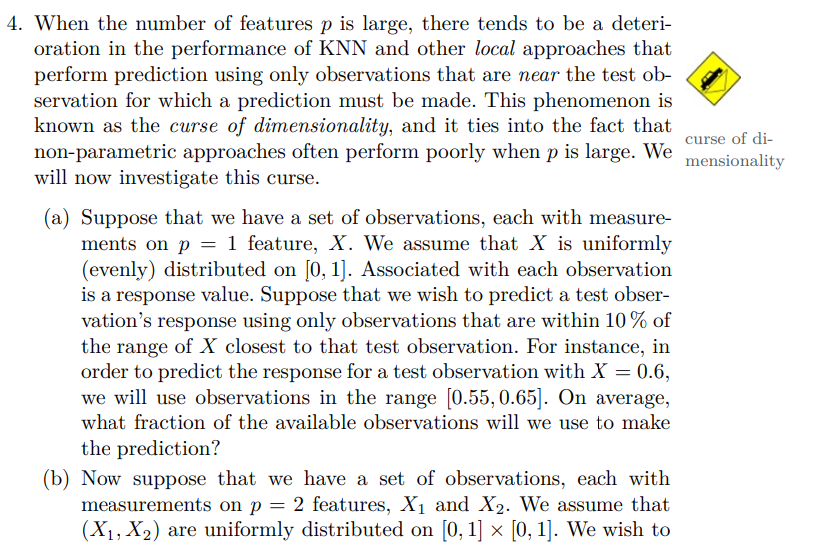
\includegraphics[width=0.71\textwidth,height=\textheight]{images/clipboard-4051626028.png}

}

\end{figure}

\begin{figure}

{\centering 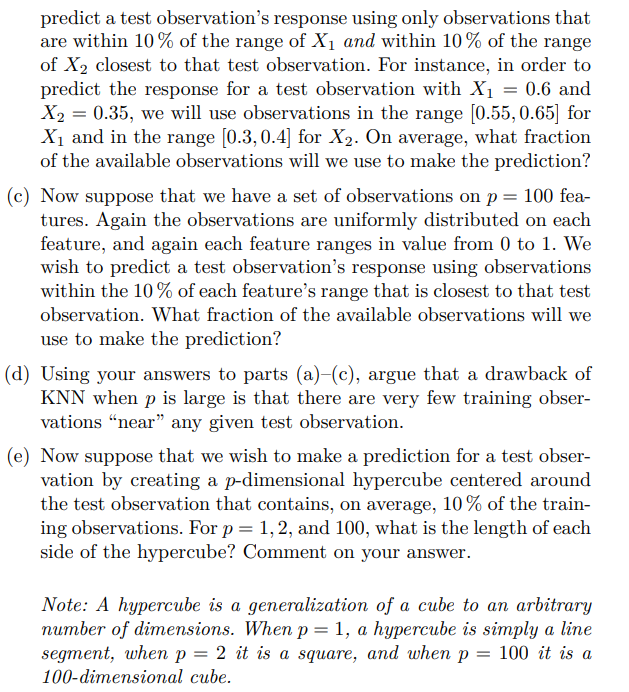
\includegraphics[width=0.6\textwidth,height=\textheight]{images/clipboard-3443800866.png}

}

\end{figure}

\begin{center}\rule{0.5\linewidth}{0.5pt}\end{center}

Solution:

(a) Since the feature \(X\) is uniformly distributed in the
range\([0,1]\), We consider a test observation and use only those within
10\% of its range.

If a test point is at \(𝑋 = 0.6\), we use observations in the range:
\([ 0.55 , 0.65]\). The total range is 1, so the fraction of data used
is\(\frac{selected\ range}{total\ range} = \frac{0.65 − 0.55}{1} = 0.1\).
Therefore, we use 10\% of the data.

(b) We now have two features, \((X_1,X_2)\), both uniformly distributed
on \([ 0 , 1] × [ 0 , 1]\).

To predict the response, we use only observations within 10\% of both
\(X_1\) and \(X_2\).

When \(X_1=0.6,\ X_2=0.35\), we will use:
\(X_1\in[0.55,0.65] ,\ X_2 \in [0.3,0.4]\).

The fraction of data used is
\(\frac{selected\ range}{total\ range} = \frac{0.10 * 0.10 }{1} = 0.01\).
Therefore, we use 1\% of the data.

(c)

Now, we have 100 features, all uniformly distributed in \([0,1]\). We
use only the observations within 10\% of each feature's range.

For each feature \(X_i\), we select observations within:
\([X_i−0.05,\ X_i+0.05]\) (assuming the test observation is not too
close to the boundaries).

Since the features are independent, the fraction of observations in each
dimension is 0.1. The fraction of data used is \((0.1)^{100}\), which is
very small number.

Therefore, in 100D space, almost none of the training data is ``close''
to the test point, making KNN ineffective.

(d)

From previous results, in 1D, we use 10\% of the data; In 2D, we use
1\%; In 100D, we use \((0.1)^{100}\), which is practically zero.

Because most points are far away, and distances between them are almost
uniform, and even with millions of points, find ``near'' neighbors is
unlikely. What's more, searching for neighbors in high-dimensional space
is inefficient.

Therefore, KNN performs poorly in high dimensions because there are too
few nearby training points, making predictions unreliable.

(e)

We define a p-dimensional hypercube centered at a test point that
contains 10\% of the total training data.

Volume of the hypercube in \(p-dimensional\) space is:
\(Fraction\ of\ Data\ Used = ( Side\ Length )^𝑝\)

Let \(s\) be the side length of the hypercube. To contain 10\% of data,
we solve: \(s^p = 0.1\).

For \(𝑝= 1\): \(s^1 = 0.1\), \(s=0.1\). In 1D, we take 10\% of the
range.

For \(𝑝= 2\): \(s^2 = 0.1\), \(s=\sqrt{0.1} \approx 0.316\). In 2D, the
square has side length around 0.316, much larger than in 1D.

For \(𝑝= 100\): \(s^{100} = 0.1\),
\(s=0.1^{\frac{1}{100}} = 10^{-0.01} \approx 0.977\). In 100D, the side
length is about 0.977, meaning almost the entire space is included.

In high dimensions, the hypercube must be almost the entire space to
contain just 10\% of the data. This confirms why KNN is ineffective in
high dimensions: Everything is ``far'' apart, so the notion of ``nearest
neighbors'' breaks down.

Thus, KNN works well in low dimensions because neighbors are meaningful.
In high dimensions, the space becomes too sparse, making KNN
ineffective.



\end{document}
